% latex article template

% cheat sheet(eng): http://www.pvv.ntnu.no/~walle/latex/dokumentasjon/latexsheet.pdf
% cheat sheet2(eng): http://www.pvv.ntnu.no/~walle/latex/dokumentasjon/LaTeX-cheat-sheet.pdf
% reference manual(eng): http://ctan.uib.no/info/latex2e-help-texinfo/latex2e.html

% The document class defines the type of document. Presentation, article, letter, etc. 
\documentclass[12pt, a4paper]{article}

% packages to be used. needed to use images and such things. 
\usepackage[pdfborder=0 0 0]{hyperref}
\usepackage[utf8]{inputenc}
\usepackage[english]{babel}
\usepackage{graphicx}
\PassOptionsToPackage{hyphens}{url}

% hides the section numbering. 
\setcounter{secnumdepth}{-1}

% Graphics/image lications and extensions. 
\DeclareGraphicsExtensions{.pdf, .png, .jpg, .jpeg}
\graphicspath{{./images/}}

\title{
	Information systems\\
	project report\\	
}
\author{
	\underline{Group members:} \\
	Bae, Magnus\\
	Bremnes, Jan Alexander Stormark\\
	Krane, Magnus\\
	Sande, Kristian Olafsen\\
	Tørresen, Håvard\\
}
\date{\today}

\hypersetup{
	colorlinks=true,
	linkcolor=black,
	filecolor=red,
	urlcolor=blue
}

\begin{document}
\maketitle
\pagenumbering{arabic}

\newpage
\tableofcontents
\newpage
\section{Introduction}


This report documents the requirement specifications of “NTNUs Ultimate Digital Learning 
platform” (NUDL), which is a proposal for an IT-system for the Norwegian University of 
Science and Technology (NTNU). NUDL proposes to digitalize some of the current processes 
involved in studies at NTNU, such as delivering a complaint on a grade, to ease the 
process for all parties involved and cut an unnecessary load of paperwork. Beyond that 
it also proposes to streamline these processes, along with the processes that are 
already digitalized, under a standardized user interface and an updated security system.

\noindent
The report will begin with an analysis of the current situation, highlighting the 
processes and problems we found most in need of rework and digitalizing. Following, there 
will be an in-depth explanation of how we propose to solve these issues, and how NUDL 
will work and respond when put to use in situations that are managed by other systems 
today.

\section{Background}
In this chapter we will present the background for this project, and review the factors that have
influenced our decisions and vision for this project. 
\section{Old system}
\subsection{Several systems}
Today's system is divided into several semi-independent systems. This is for instance StudentWeb, Eksamensweb, Innsida 2.0, It's Learning, and etc. This means that a student has to go through several systems to do something simple. If you would like to register into a new course, you would have to deal with three different systems (Figure \pageref{fig:Register-old}). If you would like to complain on the grade, you must also interact with 3 systems, some of which demands manual labour from the faculty staff (Figure \pageref{fig:Complain-old}).
\subsection{Complexity}Since the total system is divided into several sub-system, these systems are unnecessary complex and slow. Some of these systems are also:
\begin{itemize}
\item Proprietary closed source.
\item 15 year old code base.
\item Architecturally locked in to Microsoft technologies.
\item Licensing costs.
\end{itemize}This means that they are not easy to upgrade and not very modular. It also means that if we were to upgrade only parts of the current system, it will probably end up just as complex as the current system since we would have to consider the parts that is left. %finn på et bedre navn?
\section{BPMN-models}
	The following BPMN-models\cite{bpmn} describe how we view the current processes of registering to a course, and complaining on a grade, followed by our suggested changes.
All models are from a student's perspective, as that is what we found most interesting.

\subsection{registering to a course}
		
\begin{figure}[H]
    \centering
    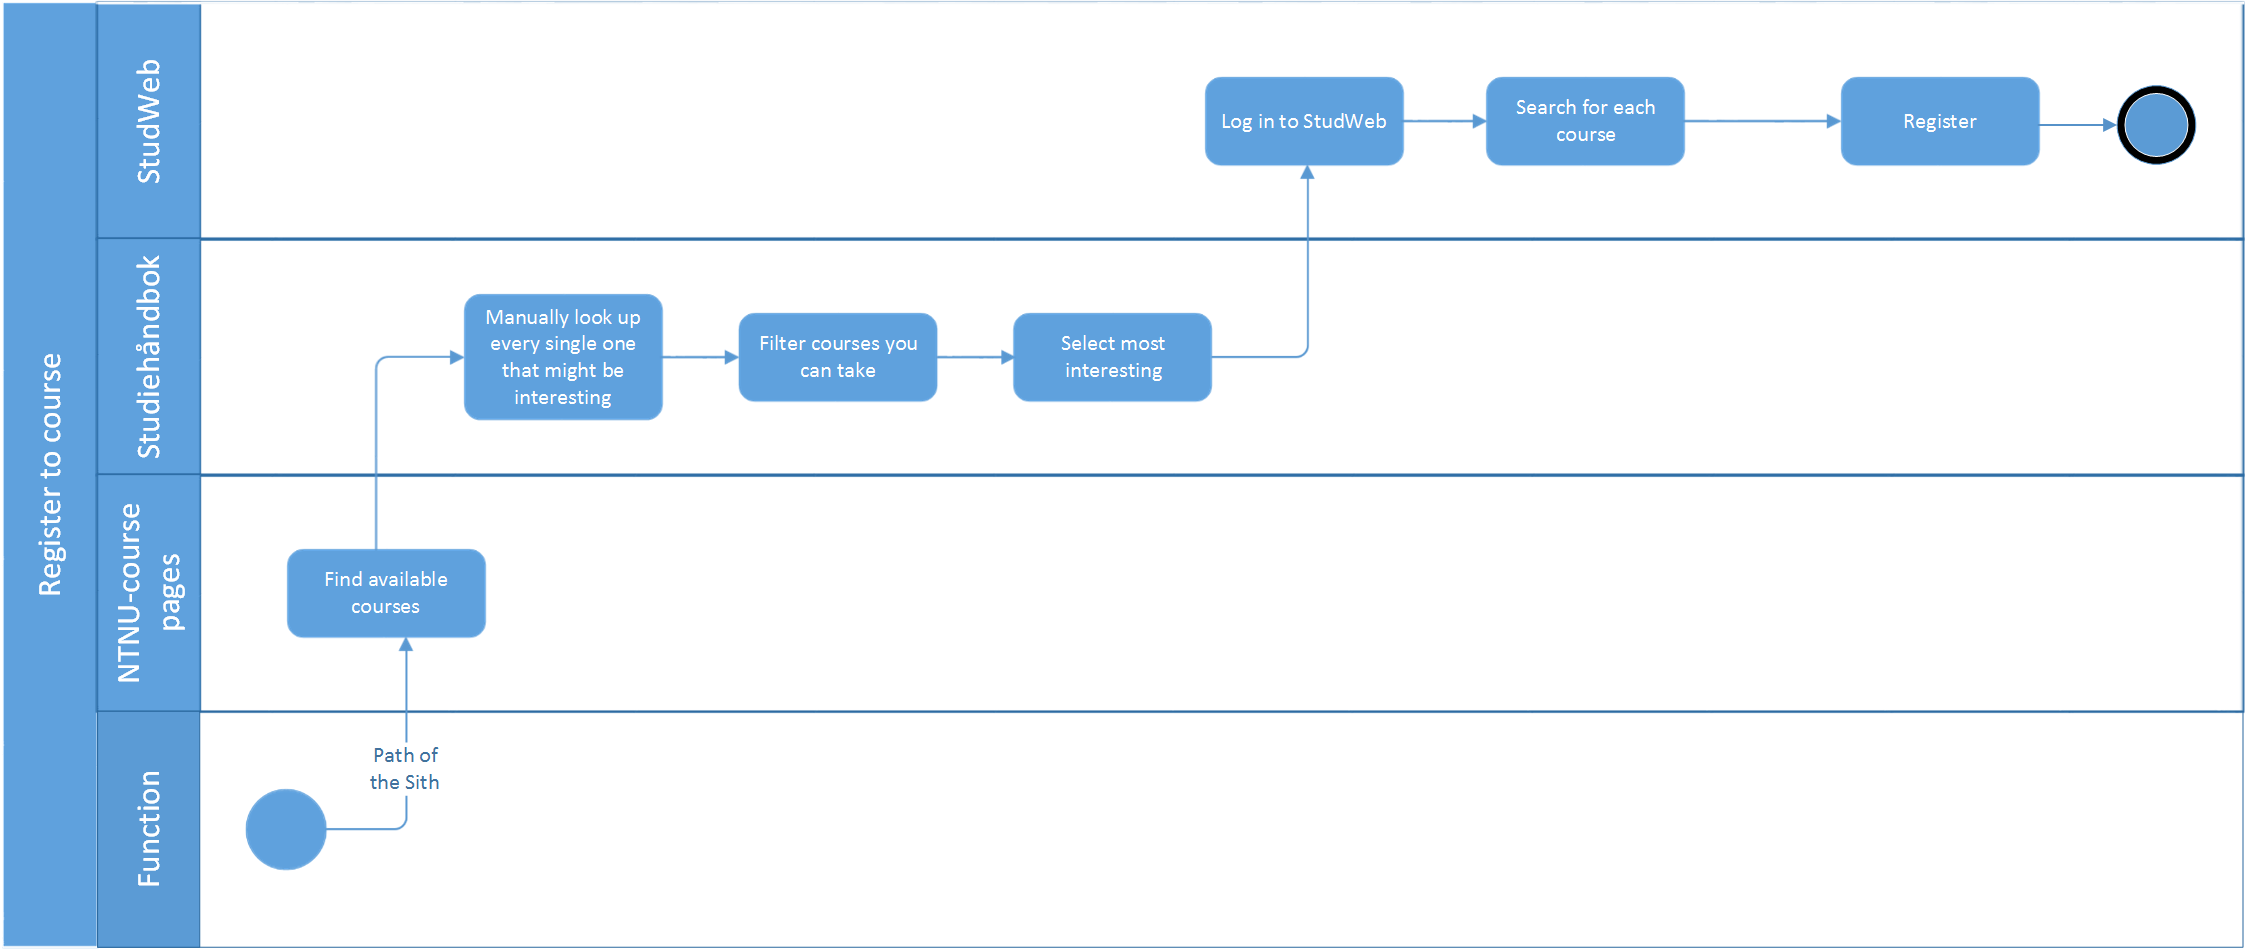
\includegraphics[width=\textheight, angle=-90]{BPMN-register-old}%apparently sets width first and then rotates
    \caption{Our interpretation of the current process of registering to a course.}
    \label{fig:Register-old}
\end{figure}

\begin{figure}[H]
    \centering
    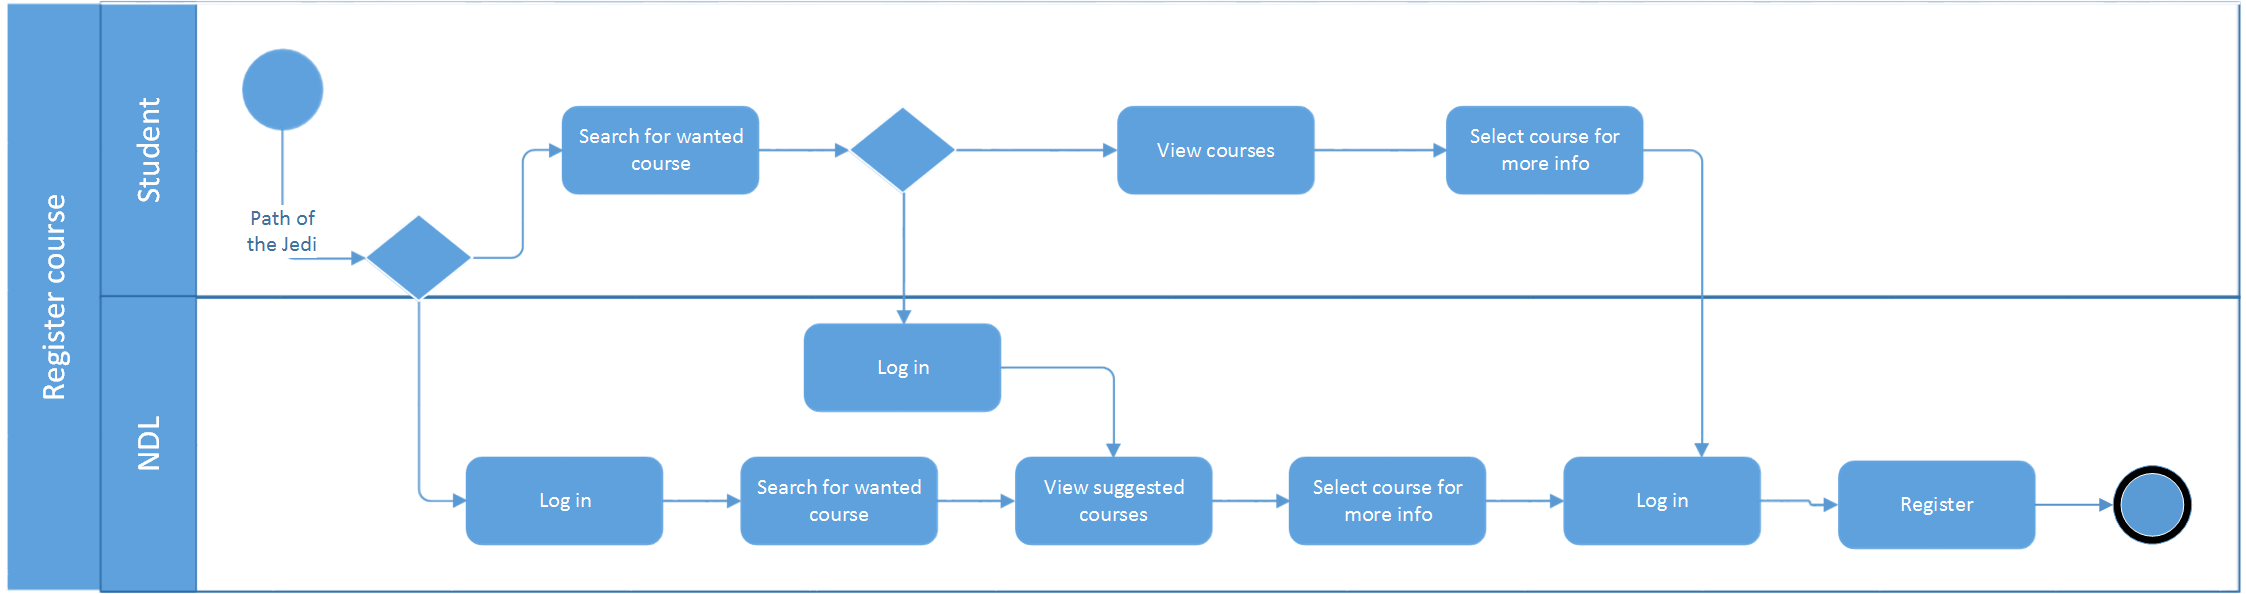
\includegraphics[width=\textheight, angle=-90]{BPMN-register}
    \caption{How we envision our new process of registering to a course to be.}
    \label{fig:Register-new}
\end{figure}

\begin{figure}[H]
    \centering
    \includegraphics[width=\textheight, angle=-90]{BPMN-complain-old}
    \caption{Our interpretation of the current process of complaining on a grade}
    \label{fig:Complain-old}
\end{figure}

\begin{figure}[H]
    \centering
    \includegraphics[width=\textheight, angle=-90]{BPMN-complain}
    \caption{How we envision our new process of complaining to be.}
    \label{fig:Complain-new}
\end{figure}

\section{How we are going to do it}
	This section will give a brief description of how we plan on implementing our solution. 
	
	\subsection{Central Datastore}
		We propose creating a central datastore containing all public information about NTNU. We will provide APIs that will give easy access to all the data, and the APIs will be open to the public. 
		% Tenk IME-API!
NUDL will use this datastore, illustrated in Figure \ref{fig:datastore}, to retrieve all necessary information about courses, rooms and timetables, and so it will need to be constantly updated in order to contain the most recent information. This means that third party developers will have equal access to non-restricted data, which will enable students and staff to write their own tools which can easily be integrated with NUDL. We aim to make NUDL a platform to which tools can be added and removed as needed, not a monolithic system where someone else is in control. The calendar generator at \url{www.ntnu.1024.no} is a great example of an extremely useful application created by a student. We know that IME offers some APIs today, and these could be extended and integrated into our system.
\begin{figure}[h]
\centering
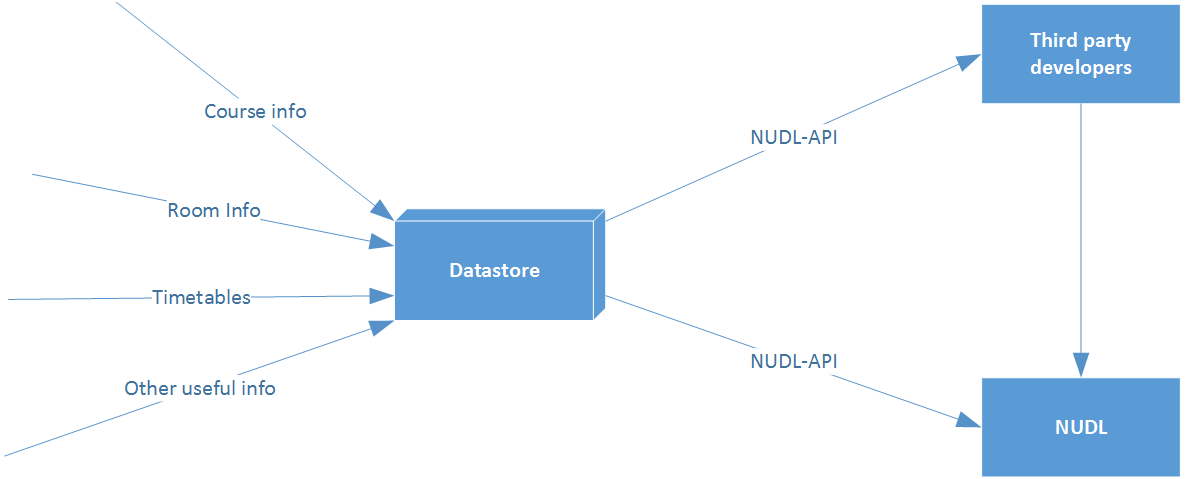
\includegraphics[width = \textwidth]{datastore}
\caption{Datastore and APIs}
\label{fig:datastore}
\end{figure}

	\subsection{Storage model}
		The datastore mentioned in the previous section will only contain publicly available information. In addition, we will have two other separate databases; one userstore containing information about staff and students, and one database storing everything related to the individual courses. In Figure \ref{fig:storagemodel} the general datastore is shown on the left, course database in the middle and userstore on the right. The dotted green circle means that everyone is given read access, a full red circle means read and write access is restricted to a strict subset of users, and a full green circle means that there are two different levels of security. The userstore will be fully secured against unauthorized access, and only the users will have access to their individual information. The course database will be used to supply the same functionality as It's Learning does today. Students will for the most part have read-only access to the course database, but they will be given the possibility to deliver exercises and participate in forums and chat. Course staff will have read and write access to the course content pages, but will only be able to read the student submissions. Administrative staff will have accesses as needed. 
Course staff will be able to make course material available to non-students, by making it accessible through the public APIs. 
\begin{figure}
\centering
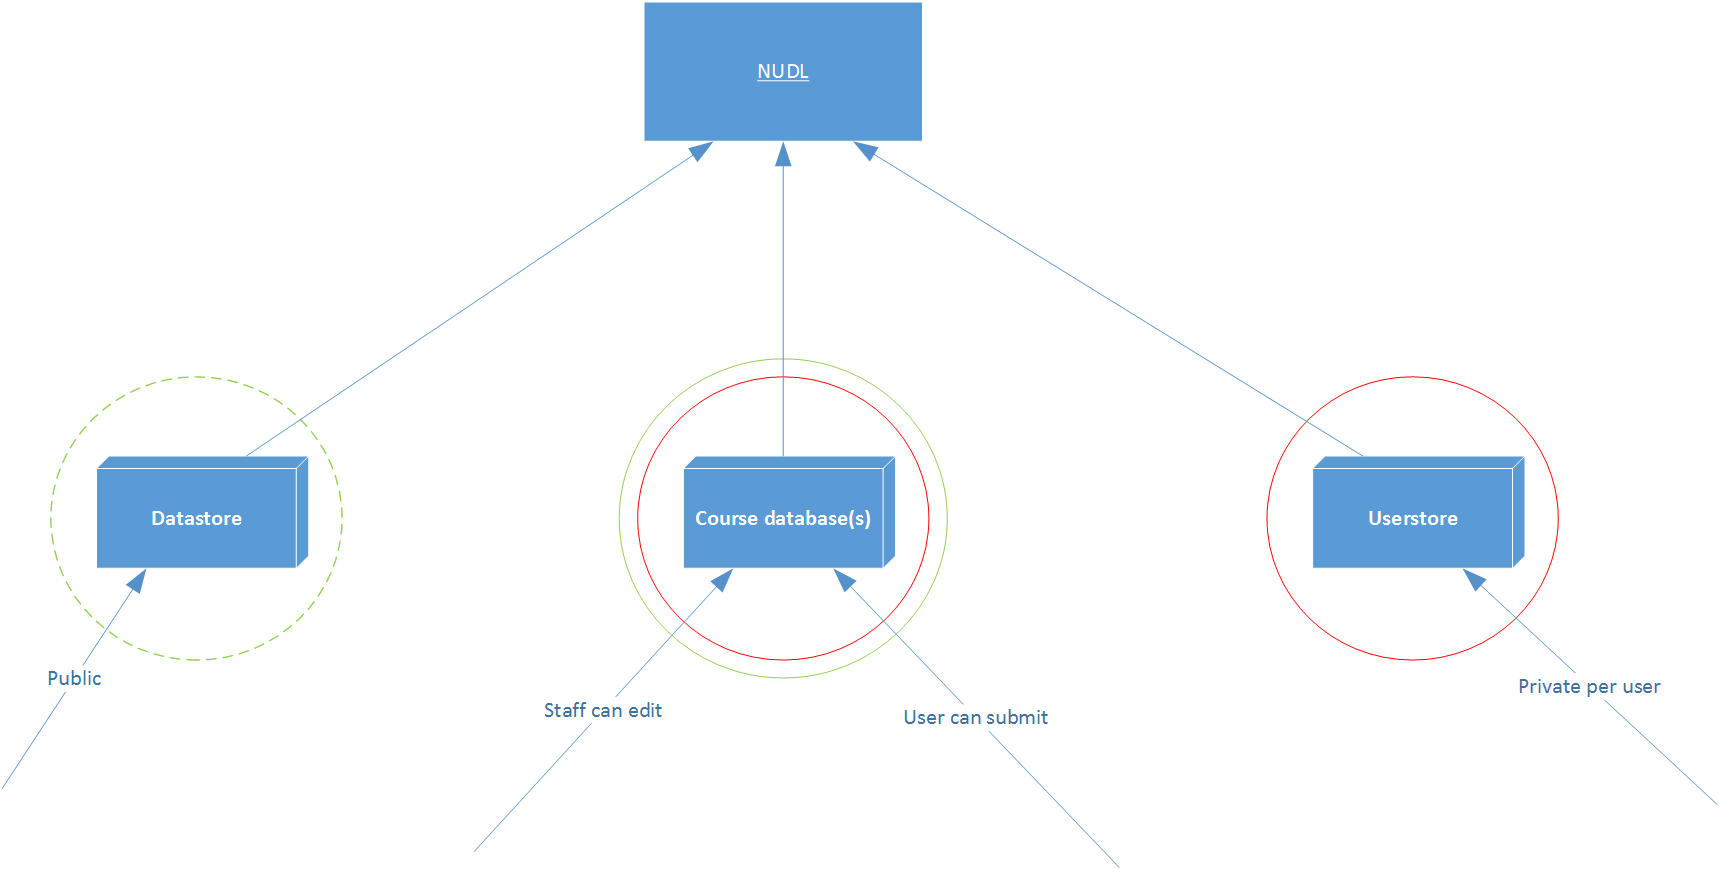
\includegraphics[width = \textwidth]{moreStorage}
\caption{Storage model}
\label{fig:storagemodel}
\end{figure}

		
	\subsection{User interface} 
		We want NUDL to present users with a user-friendly and unified interface. It will not be like today, where you have different interfaces for It's Learning, Studweb and Eksamensweb. It's Learning and Eksamensweb will be replaced by NUDL, and Studweb will be hidden from view. Students can log in to Studweb from NUDL, via Feide, but they will be met by the NUDL interface, which will take care of the communication with Studweb, as shown in Figure \ref{fig:layers}. Staff and students can do everything they need to do, from one central location. There will be no more need to log in to different services like today, where one first has to search for courses on ntnu.no, (UI no.1) log on to Studweb in order to register for the course (navigating a very cluttered and confusing UI no.2) and then log on to Innsida (UI no.3) and then finally continue to It's Learning (UI no.4). If they want to complain on a grade, they need to send in a paper form, or students at IDI can log on to Eksamensweb (UI no.5). NUDL combines all these different interfaces into one coherent whole. 
\begin{figure}
\centering
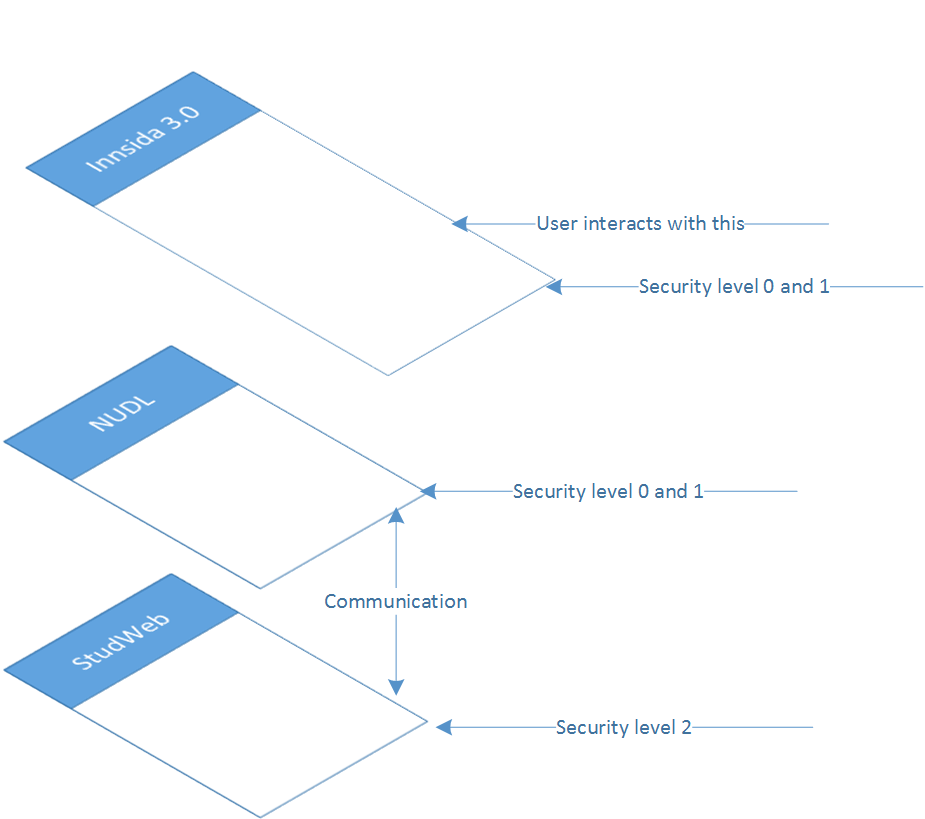
\includegraphics[width = \textwidth]{Layers}
\caption{Layered architecture}
\label{fig:layers}
\end{figure}

\bibliography{bibliography}
\bibliographystyle{acm}

\end{document}
